\chapter{Basic Colour Strategy}
\label{s:basic-strategy}
\label{s:first-strategy}
\is{language strategy!for colour!basic colour strategy}
\is{basic colour strategy|see{language strategy}}

The \emph{basic colour strategy} is by far the most studied language
strategy for the domain for colour. It stipulates that a colour should
be described using a single colour term that refers to a single colour
category. At the semantic level it specifies how the categorisation
process should be organised; at the syntactic level it specifies how
these categories should be expressed in language. As this strategy has
been studied extensively in the domain of artificial language
modelling, it allows me to establish a solid common base before moving
on to the other strategies.

\section{Related research}

\subsection{Colour categories}

Colour categories\is{colour category} are considered to be
prototypical in nature \citep{rosch73natural}. One colour sample, the
\emph{prototype}\is{prototype|see{colour category}}, is considered
to be the best example of a certain category and membership to this
category is graded: some samples are considered to be better members
of a certain category than others. A bluish shade of green is for
example considered to be a worse example of the category of green than
the natural colour of grass.

\subsubsection*{Determining location of basic colour categories}

Part of the research in colour cognition aims at locating the typical
member of each colour category of the category systems in different
natural languages, such as Spanish \citep{lillo07locating}, English
\citep{boynton87locating, sturges95location} and Russian
\citep{safuanova07russian}. These experiments typically involve naming
a set of individual colour samples.

In colour literature, the distinction is made between the \emph{focus}
(the colour sample which is named fastest) and the \emph{centroid}
(the colour central to all colours that belong to the category) of a
colour category. Interestingly, a discrepancy exists between the
locations of these two \citep{sturges95location}. Some of the
experiments also reported on \emph{consensus samples}\is{consensus
  samples|see{colour category}}, which are samples that were
consistently named by all participants in the experiment. The
consensus samples for English \citep{sturges95location} are shown in
Figure \ref{f:basic-consensus-chips-english}.

\begin{figure}[htbp]
  \begin{center}
    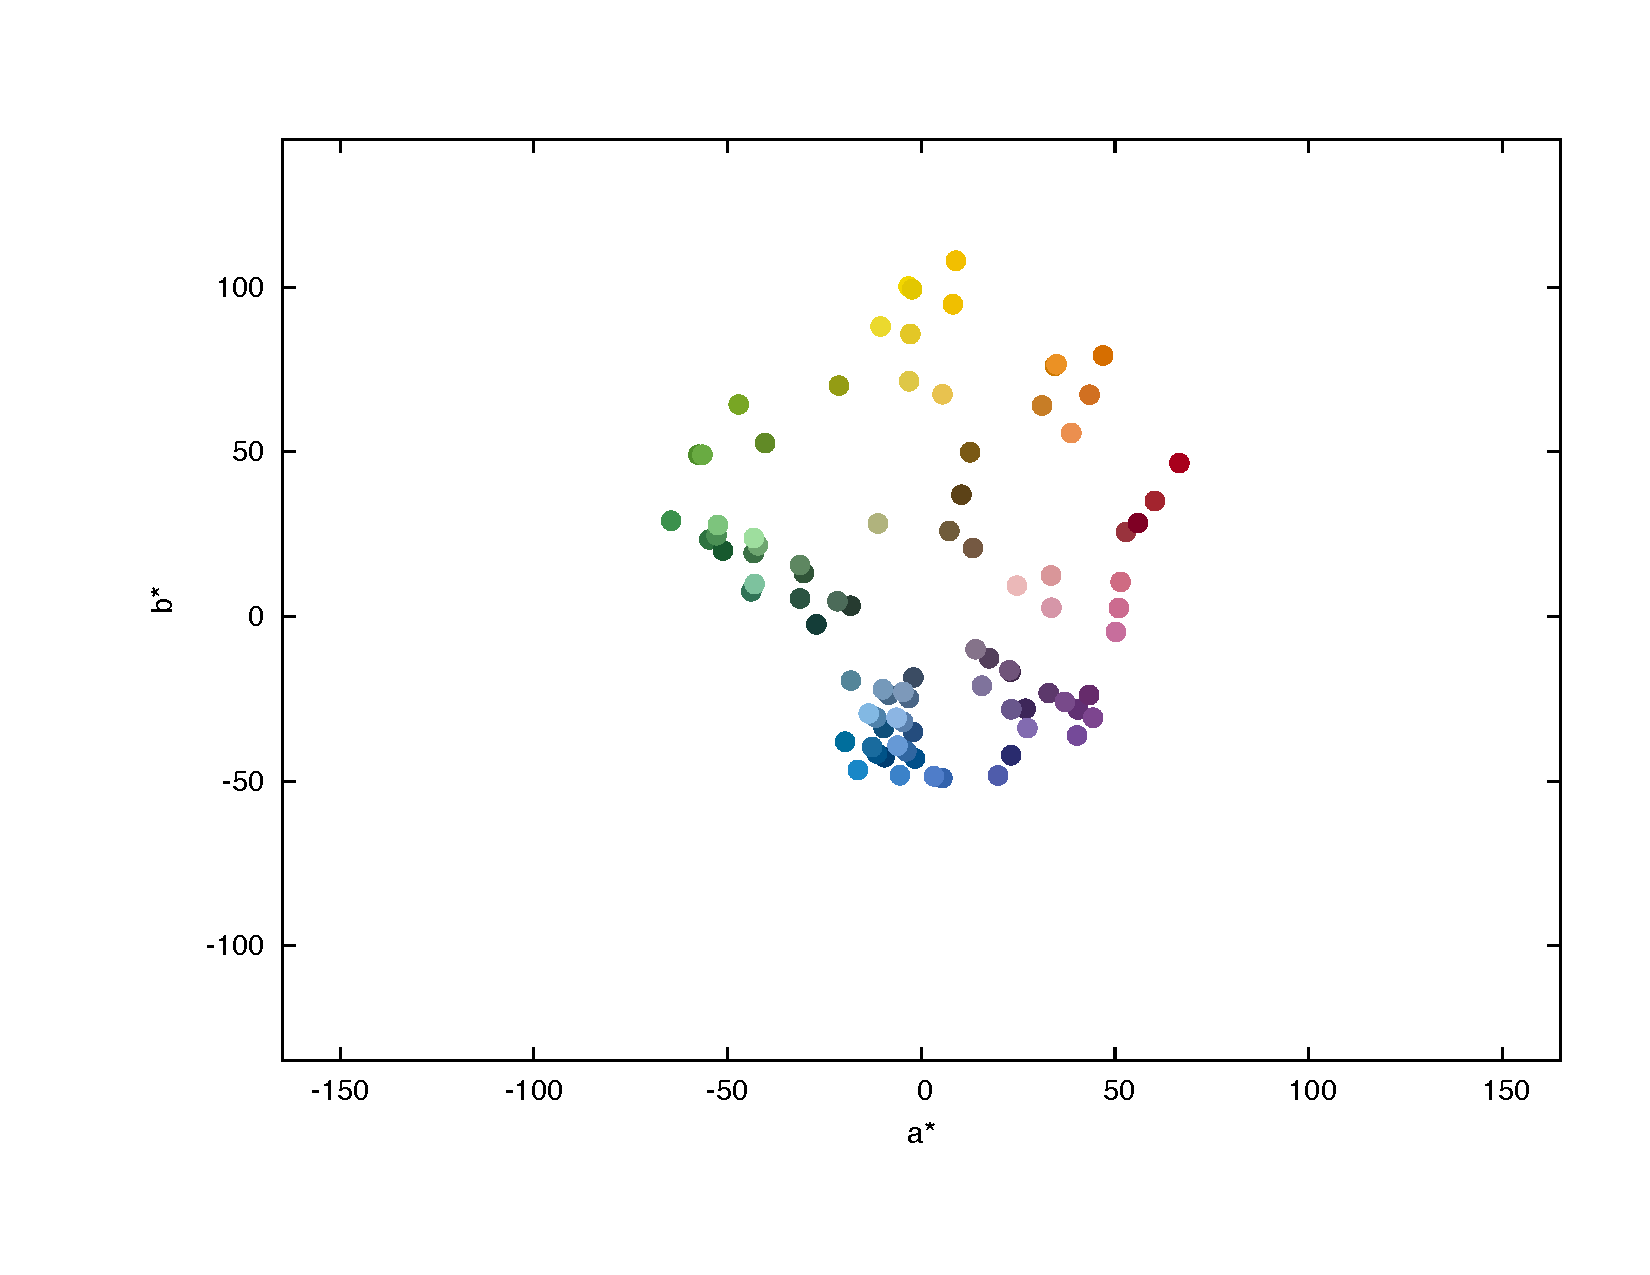
\includegraphics[width=.85\textwidth]{./basic-strategy/figures/sturges-consensus-chips.pdf}
    \caption[Consensus chips for English]{The consensus chips (all
      samples that were consistently named by all participants) for
      English \citep{sturges95location}.}
    \label{f:basic-consensus-chips-english}
  \end{center}
\end{figure}

\subsection{Models}

The \emph{basic colour strategy} has received quite some attention
within the field of artificial language evolution. Most of these
studies adhere to the the language game paradigm and use the colour
naming game (see Section \ref{s:language-games-for-colour}) to study
how a population of agents could coordinate their own colour category
system. Although there seems to be a high coherence in the models that
have been proposed for this game, different implementation choices
have been made. Colour categories were represented either as radial
basis function networks \citep{steels05coordinating}, single points in
a three dimensional conceptual space \citep{belpaeme05explaining,
  belpaeme07language} or a set of points sharing the same linguistic
label in a one dimensional conceptual space \citep{puglisi08cultural,
  baronchelli10modeling}. A comparison between the different
implementations of the \emph{basic colour strategy} is shown in Table
\ref{t:language-game-models-comparison}.

\renewcommand{\arraystretch}{1.5}
\begin{table}[htbp]
\resizebox{\textwidth}{!}{
%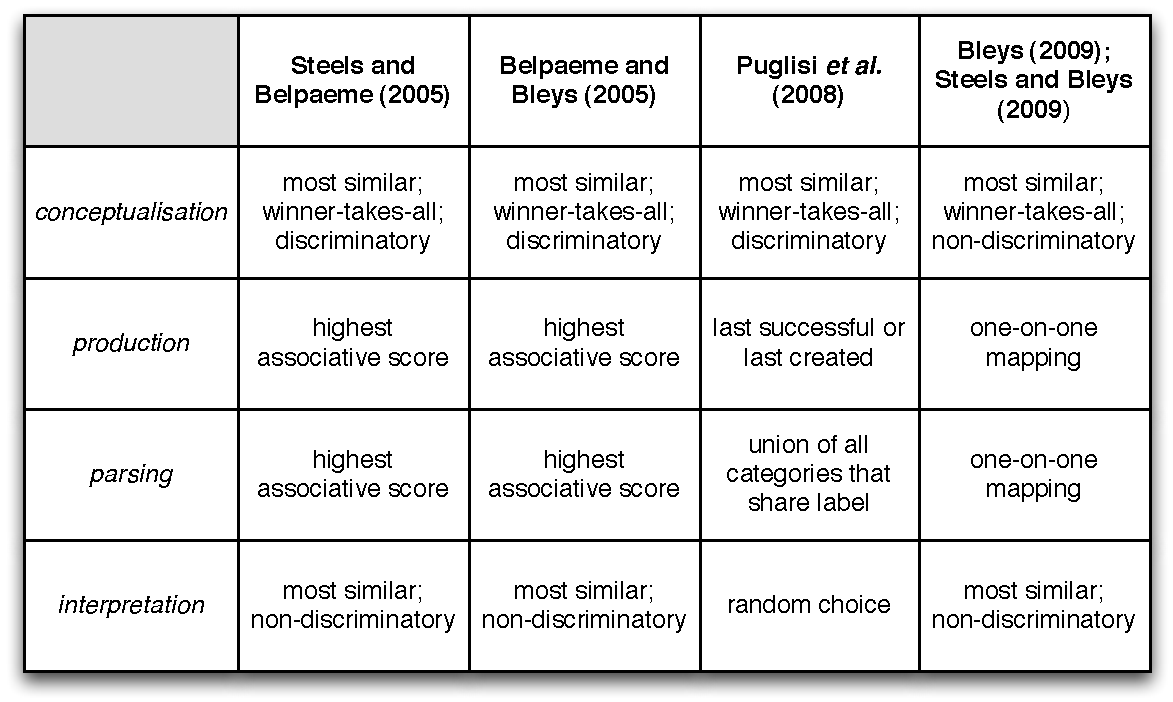
\includegraphics[width=\textwidth]{./basic-strategy/figures/language-game-models-comparison}
  \begin{tabular}{>{\centering\arraybackslash}m{.2\textwidth}>{\centering\arraybackslash}m{.275\textwidth}>{\centering\arraybackslash}m{.275\textwidth}>{\centering\arraybackslash}m{.275\textwidth}>{\centering\arraybackslash}m{.275\textwidth}}
  \lsptoprule
  & \citet{steels05coordinating} & \citet{belpaeme05explaining} & \citet{puglisi08cultural} & Bleys (2009);\newline \citet{bleys09linguistic} \\
  \midrule
  \textsc{conceptual\-isation} & most similar; winner-takes-all; discriminatory & most similar; winner-takes-all; discriminatory & most similar; winner-takes-all; discriminatory & most similar; winner-takes-all; non-discriminatory \\
  \textsc{production} & highest associative score & highest associative score & last successful or last created & one-on-one mapping \\
  \textsc{parsing} & highest associative score & highest associative score & union of all categories that share label & one-on-one mapping \\
  \textsc{inter\-pretation} & most similar; non-discriminatory & most similar; non-discriminatory & random choice & most similar; non-discriminatory \\
  \lspbottomrule
  \end{tabular}
 }
  \caption[Comparison of the different models for the basic colour
  strategy]{Comparison of the different models for the basic colour
    strategy.}
  \label{t:language-game-models-comparison}
\end{table}
\renewcommand{\arraystretch}{1}


\section{Semantic template}
\label{s:bs-semantic-template}
\is{semantic template!for basic colour strategy}

In previous models of the colour naming game
\citep{steels05coordinating, belpaeme05explaining, puglisi08cultural}
the speaker selected the category that was most similar to the topic
entity. Additionally this category needed to be discriminatory in the
current context: no other entity in the context should be categorised
as belonging to the same category as the topic. In general, the hearer
was more lenient: it selected the entity that was most similar to the
interpreted category, regardless of whether it would actually be
classified as the interpreted category and whether other entities
would be classified as the same category. So for example, the hearer
would select an orange entity when interpreting the yellow colour
category even if it would know a colour category for orange. Previous
research has shown the negative impact of applying the discriminatory
criterion as a hearer, especially when the category systems of the
agents are not aligned \citep{belpaeme07language}.

The semantics I propose in this book adhere to the main ideas
proposed by the previous models, but with a minor difference. The
speaker still selects the category that is most similar to the topic
entity and the hearer will point to the entity that is most similar to
the interpreted category. The speaker however is a bit more lenient as
it does not apply the discriminatory criterion. This will result in a
higher level of communicative success, as the speaker will now be able
to successfully name entities that are most similar to a category,
even if this category is not discriminatory. For example, if the
context contains two green colour samples, the sample that is most
similar to the green colour category can still be successfully
named. 

The semantic template of the \emph{basic colour strategy} can be
summarised in three steps: profiling, categorisation and
selection. These processes are represented separately in semantics as
this will enhance possible re-use of these primitives in other
strategies.

\subsection{Profiling}
\is{profiling}

During the categorisation process, some dimensions of the colour
domain might have a bigger impact than others (see Section
\ref{s:intro-basic-colour-strategy}). In order to represent this in
semantics, I need primitives that will \emph{profile}, or highlight,
some dimensions of a particular colour sample before the
categorisation process. For each strategy reported in the literature
review, I define a different primitive.

This profiling could also instruct the vision system of a robotic
agent to process the colour information of the objects. This could
defer the computation of the different features of the objects until
they become absolutely necessary.

\subsection{Categorisation based on colour}
\label{s:bcs-categorisation}

As the main psychological theory for categorisation, I have chosen to
follow the prototype-based approach to colour categories as advocated
by \cite{rosch73natural}. In this theory, a category is defined by its
prototype. This prototype serves as the best sample of a category and
is compared to a particular colour sample to determine the graded
membership of this sample to this category.

Both colour samples and prototypes of colour categories are
represented in the CIE $L^*a^*b^*$ (see Section \ref{s:lab}) colour
space. This colour space turned out to be the best space in a related
model of colour naming \citep{lammens94computational} and is
\emph{equidistant}: Euclidean distance between colours represented in
this space reflects psychological differences as perceived by humans.

Similarity can thus be expressed as an exponentially decaying function
\citep{shepard87toward, gardenfors04conceptual} of the weighted
distance between the prototype of a colour category and a colour
sample (as shown in Equation \ref{e:similarity}). In this function,
$c$ is a sensitivity parameter. As in the current simulations this
parameter is identical for all colour categories, the actual value of
this parameter does not result in any qualitatively different
results. It is possible to imagine simulations in which the
sensitivity parameter is different for each colour category, so that some 
categories cover a relative larger area of the
colour space than others. The distance is weighted in each dimension by the
product of the current profile of the entity and the weights of the
prototype of the colour category. The weights of a prototype reflect
the importance of each dimension for that category. Some categories,
such as the basic colour categories, are defined in all dimensions,
whereas others are only defined in some dimensions (such as the
lightness dimension for the categories for light and dark). The exact
equation is shown in Equation \ref{e:weighted-distance}.

\begin{align}
s(i,j) &= e^{-cd_w(i,j)}
\label{e:similarity} \\
d_w(x,y) &= \sqrt{\sum_{k=1}^n w_{x_k}w_{y_k} (x_k - y_k)^2}
\label{e:weighted-distance}
\end{align}

\subsection{Selection based on activation}

An activation value is assigned to each entity, which reflects the
similarity of that entity to the category that was used during the
categorisation process. The more similar the entity was to the
category, the higher the activation will be. The entity with the
highest activation will be selected as the outcome of the complete
process.

\subsection{Semantic constraint network}

The semantic constraint network for the \emph{basic colour strategy} is shown
in Figure \ref{f:bcs-semantic-structure}. The {\sc
  Equal-to-Context} primitive introduces all entities in the sensory
context of the agent. The {\sc Profile-Colour-Dimensions} primitive
sets the focus to each entity in the context based on the dimension
profiler that is bound to its third slot. The {\sc
  Filter-by-Colour-Lenient} primitive performs the categorisation
process based on the colour categories known to the agent and assigns
an activation score of the remaining entities. Finally, {\sc
  Select-Most-Activated} selects the entity with the highest
activation from the set of activated entities.

Whether the {\sc Filter-by-Colour-Lenient} primitive selects a subset
of entities from its input set depends on whether the argument for its
colour category is already bound. During conceptualisation, the
argument for the colour category will typically be unbound and hence
the primitive will divide the entities of the context in different
subsets. In interpretation however, the colour category is already
known and will be used to set the activation of all the entities in
the context.

\begin{figure}[htbp]
  \begin{center}
    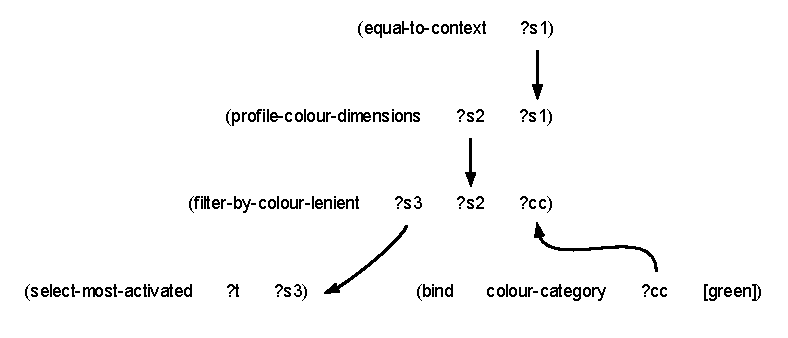
\includegraphics[width=\textwidth]{./basic-strategy/figures/semantics-interpretation.pdf}
    \caption[The semantic constraint network for the basic colour
    strategy]{The semantic constraint network for the basic colour
      strategy. The {\sc Profile-Colour-Dimensions} primitive profiles
      some dimensions in the context. {\sc Filter-by-Colour-Lenient}
      performs the the categorisation process and assigns activation
      values to the entities. The {\sc Select-Most-Activated}
      primitive will select the entity with the highest activation.}
    \label{f:bcs-semantic-structure}
  \end{center}
\end{figure}

\subsection{Semantic primitives}

\definition{Semantic Primitive}{Equal-to-Context}

\begin{explanation}{description}
Retrieves all entities from in the sensory context and collects them in an entity set.
\end{explanation}

\begin{explanation}{arguments}
\verb+?context+ (of type entity-set)
\end{explanation}

\begin{explanation}{revision specs}
$\emptyset$: collects all entities in the sensory context in an entity set and binds it to \verb+?context+
\end{explanation}

\definition{Semantic Primitive}{Profile-Colour-Dimensions}

\begin{explanation}{description}
Profiles the colour dimensions of the entities in an entity set.
\end{explanation}

\begin{explanation}{arguments}
\verb+?profiled-set+ (of type entity-set) \\
\verb+?source-set+ (of type entity-set)
\end{explanation}

\begin{explanation}{revision specs}
  \verb+?source-set+: profiles all colour dimensions of the entities
  in the entity set and binds the resulting entity-set to
  \verb+?profiled-set+
\end{explanation}

\begin{explanation}{note}
  Other variants of this primitive which profile other dimensions are
  defined as well. {\sc Profile-Brightness-Dimension} profiles only in
  the $L^*$ dimension and {\sc
    Profile-Brightness-and-Red-Green-Dimensions} profiles both the
  $L^*$ and $a^*$ dimension.
\end{explanation}

\definition{Semantic Primitive}{Filter-by-Colour-Lenient}

\begin{explanation}{description}
  Applies a colour category to a set of entities. When the colour
  category is known, this primitive sets the activation of each entity
  in the set to the similarity between the entity and the
  category. When the colour category is unknown, it categorises the
  entities in the set to the category that is most similar to it.
\end{explanation}

\begin{explanation}{arguments}
\verb+?categorised-set+ (of type entity-set) \\
\verb+?source-set+ (of type entity-set) \\
\verb+?colour-category+ (of type colour-category)
\end{explanation}

\begin{explanation}{revision specs}
  \verb+?source-set ?colour-category+: sets the activation of the
  entities in the source set to the similarity to the colour category
  and binds the resulting entity-set to \verb+?categorised-set+ \\
  \verb+?source-set+: categorises each entity in the source set to the
  category that is most similar to it and returns pairwise bindings
  for \verb+?colour-category+ and \verb+?categorised-set+
\end{explanation}

\definition{Semantic Primitive}{Select-Most-Activated}

\begin{explanation}{description}
Selects the entity from an entity-set that has the highest activation.
\end{explanation}

\begin{explanation}{arguments}
\verb+?entity+ (of type entity) \\
\verb+?entity-set+ (of type entity-set)
\end{explanation}

\begin{explanation}{revision specs}
\verb+?entity-set+: selects the entity from the entity-set with the highest activation and binds it to \verb+?entity+
\end{explanation}

\section{Syntactic templates}
\label{s:bcs-syntactic-templates}

The next question I have to address is how these semantic constraint
networks will be expressed in a serial utterance. When the hearer
parses this utterance, it should be able to fully reconstruct the
constraint network that the speaker wanted to transfer. 

The main approach adopted to express semantic networks in language is
outlined as follows. The semantic network is divided in three layers
of units: (a) entity units containing the semantic entities, (b)
functional units which make direct use of such a semantic entity and
(c) contextual units which contain any remaining operations of the
semantic constraint network that do not make direct use of any
semantic entity. This division is illustrated in Figure
\ref{f:bcs-linguistic-structure}.

\begin{figure}[htbp]
  \begin{center}
    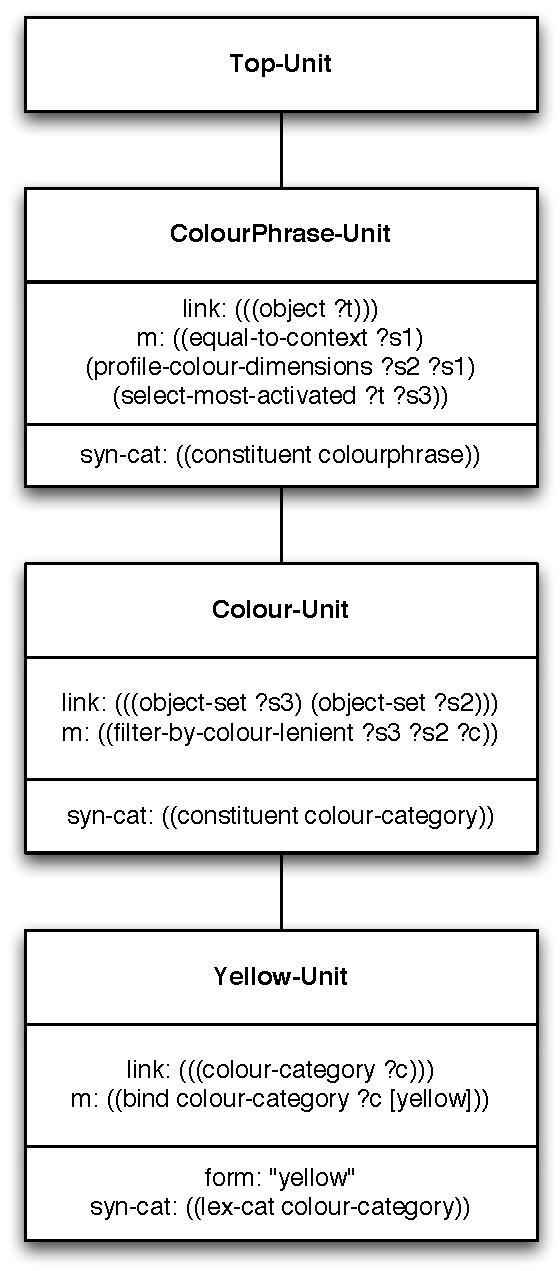
\includegraphics[width=.45\textwidth]{./basic-strategy/figures/linguistic-structure.pdf}
    \caption[Example linguistic structure for basic colour
    strategy]{Example linguistic structure for \texttt{colour-network
        1}. The semantic constraint network is divided over three
      layers of units: one for the semantic entity [yellow], one for
      the functional primitive \textsc{Filter-by-Colour-Lenient} and
      one contextual unit for all other primitives of the semantic
      constraint network. The link feature links the variables for the
      entities and entity-set. Similarly, the c-link feature passes
      the variables for colour categories and sets of colour
      categories.}
    \label{f:bcs-linguistic-structure}
  \end{center}
\end{figure}

As a rule of thumb, the reader can assume that each rule introduces
one new unit in the linguistic structure. In production, syntactic
information is added to the structure: which words will be used to
express certain semantic entities, to which syntactic category does
each unit belong and which word order should be applied when this tree
is transformed into an utterance. During interpretation, each word in
the utterance introduces a new semantic entity. Based on the lexical
categories of these entities, the hearer is able to add the layer of
functional units. Finally, the information on the word order
constraints augmented with the information of the syntactic categories
allows the agent to select the right contextual rule. This rule adds
extra primitive constraints to the network, but more importantly also
connects all primitive constraints by introducing variable equalities
(for example between the first argument of
\textsc{Filter-by-Colour-Lenient} and the second argument of
\textsc{Select-Most-Activated}) in the network shown in Figure
\ref{f:bcs-semantic-structure}.

The syntactic templates specify the rules to express a semantic
network in a serial utterance. I will now discuss each step in more
detail. Three templates (1.1 to 1.3) take care of creating the rules
that ensure the default division in three layers of units: (a) entity
units containing the semantic entities, (b) functional units which
contain primitives that make direct use of such a semantic entity and
(c) contextual units which contain any other primitives that do not
make direct use of semantic entities.

\subsection{Syntactic template 1.1: Semantic entities}
\is{syntactic template!for semantic entities}

A semantic entity is an entity from the ontology used by a primitive,
such as a category, a prototype, a relation, etc. They have an
identifier which is created when the entity itself is constructed and
which can be used in a lexical rule. In parsing, the resulting rule
will also introduce a new variable that will allow the entity to be
used by other primitives in the network. To ensure this linking is
possible, the variable needs to be part of the link feature of that
unit.

An example of a lexical rule for the colour category yellow is given
below. The main association is between the category for yellow and the
string ``yellow''. Additionally, the rule adds a link feature to the
semantic side that enables other units to incorporate this semantic
entity in the rest of the semantic network. This rule is responsible
for introducing the Yellow-Unit in Figure
\ref{f:bcs-linguistic-structure} both in production and in parsing.

\footnotesize
\begin{Verbatim}[frame=lines, label=Entity rule for yellow]
((?top-unit
  (tag ?meaning 
       (meaning ((bind colour-category ?c [yellow])))))
 ((J ?yellow-unit ?top-unit)
  ?meaning
  (link (((colour-category ?c))))))
<-->
((?top-unit
  (tag ?form 
       (form ((string ?yellow-unit "yellow")))))
 ((J ?yellow-unit ?top-unit)
  ?form
  (syn-cat ((lex-cat colour-category)))))
\end{Verbatim}
\normalsize

\subsection{Syntactic template 1.2: Functional primitives}
\is{syntactic template!for functional primitives}
\is{functional primitive|see{primitive constraint}}
\is{primitive constraint!functional primitive}

\emph{Functional units}, created by \emph{functional rules}, handle
the primitives in a semantic network that directly use a semantic
entity. For each such primitive a separate functional rule is
created. The template to express such a primitives has a subunit for
each of its arguments. The functional unit that will be introduced by
this rule contains the functional primitive that needs to be covered.
As the other arguments of the primitive are not provided by the entity
unit, these arguments become available in the link of the new
functional unit. This link ensures the encapsulated primitive can be
incorporated in a larger semantic network.

An example of such a rule for the \textsc{Filter-by-Colour-Lenient}
primitive is given below. It uses a colour-category $?c$ , for example
the prototype for yellow, from the set of colour categories $cs$ to
filter some elements from a source set $?s2$ to yield a subset of
blocks $?s1$. It associates this primitive to a newly invented
syntactic constituent category (constituent colour-category).  The
variable of the colour category is linked in through the link feature 
specified in the subunit. The new unit will have the two object-sets,
$?s1$ and $?s2$, as values for the link feature 
as these yet need to be covered by
another rule. The resulting rule is shown below.

\footnotesize
\begin{Verbatim}[frame=lines, label=Functional rule for Filter-by-Colour-Lenient]
((?top-unit
  (sem-subunits (?colour-category-unit)) 
  (tag ?meaning
       (meaning ((filter-by-colour-lenient ?s3 ?s2 ?c)))))
 (?colour-category-unit 
  (link (((colour-category ?c)))))
 ((J ?filter-by-colour-unit ?top-unit (?colour-category-unit))
  ?meaning
  (link (((entity-set ?s3) (entity-set ?s2))))))
<-->
((?top-unit 
  (syn-subunits (?colour-category-unit)))
 (?colour-category-unit 
  (syn-cat ((lex-cat colour-category))))
 ((J ?filter-by-colour-unit ?top-unit (?colour-category-unit))
  (syn-cat ((constituent colour-category)))))
\end{Verbatim}
\normalsize

\subsection{Syntactic template 1.3: Contextual primitives}
\label{s:bcs-contextual-primitive}
\is{syntactic template!for contextual primitives}
\is{contextual primitive|see{primitive constraint}}
\is{primitive constraint!contextual primitive}

The primitives that do not make direct use of semantic entities are
grouped together in a \emph{contextual unit}. This unit is introduced
by the application of a \emph{contextual rule}, which contains
subunits for each of the functional primitives. It uses the link
feature of each of its subunits to ensure the primitives will be
incorporated in the primitives it contains. The unit that is
introduced will have as link feature the target entity of the semantic
constraint network it captures.

An example of such a rule for the contextual primitives of the
semantic network shown in Figure \ref{f:bcs-semantic-structure} is
given below. It encapsulates three primitives,
\textsc{Equal-To-Context}, \textsc{Profile-Colour-Dimensions} and
\textsc{Select-Most-Activated}. It requires one subunit to be present
in the structure which belongs to the syntactic category Constituent
Colour-Category and which has as link feature of two object sets. In
parsing, it will ensure the variables in these links are made equal to
the variables of the semantic primitives it contains. The newly
introduced unit will be of a newly invented syntactic category,
Constituent ColourPhrase, and will have as link feature the first
argument of the \textsc{Select-Most-Activated} primitive.

\footnotesize
\begin{Verbatim}[frame=lines, label=ColourPhrase rule for Basic Colour Strategy]
((?top-unit
  (sem-subunits (?colour-unit))
  (tag ?meaning
       (meaning ((select-most-activated ?t ?s3)
                 (profile-colour-dimensions ?s2 ?s1)
                 (equal-to-context ?s1)))))
 (?colour-unit
  (link (((entity-set ?s3) (entity-set ?s2)))))
 ((J ?colourphrase-unit ?top-unit (?colour-unit))
  ?meaning
  (link (((colour-entity ?t))))))
<-->
((?top-unit 
  (syn-subunits (?colour-unit)))
 (?colour-unit 
  (syn-cat ((constituent colour-category))))
 ((J ?colourphrase-unit ?top-unit (?colour-unit))
  (syn-cat ((constituent colourphrase)))))
\end{Verbatim}
\normalsize

\section{Baseline experiment}
\label{s:basic-baseline-experiment}
\is{baseline experiment!for basic colour strategy}

A first test whether the proposed templates are valid is provided by a
naming benchmark\is{naming benchmark!for basic colour strategy}. It
involves naming all consensus chips for English
\citep{sturges95location} and verifying whether the resulting names
corresponds to those reported in literature. This benchmark is only
performed for the language system that is based on the centroids of
English \citep{sturges95location}. The results are shown in Table
\ref{t:bcs-naming-benchmark}. The benchmark reaches only around 83\%
success.  This suggests that, although capable of accounting for more
than three quarters of the consensus chips, the one-nearest neighbour
classification algorithm might be too general to capture all the
richness of human colour categories.

\begin{table}[htbp]
  \centering
  \resizebox{.85\textwidth}{!}{
  \begin{tabular}{rrrrrrrrrrrr}
    \lsptoprule
    \multicolumn{1}{c}{\scshape we} & \multicolumn{1}{c}{\scshape gy} & \multicolumn{1}{c}{\scshape bk} & \multicolumn{1}{c}{\scshape gn} & \multicolumn{1}{c}{\scshape yw} & \multicolumn{1}{c}{\scshape bl} & \multicolumn{1}{c}{\scshape rd} & \multicolumn{1}{c}{\scshape pu} & \multicolumn{1}{c}{\scshape br} & \multicolumn{1}{c}{\scshape or} & \multicolumn{1}{c}{\scshape pk} & \scshape total\\
    \midrule
    2 & 6 & 3 & 22 & 8 & 25 & 4 & 14 & 4 & 6 & 6 & 100 \\
    \midrule
    2 & 6 & 3 & 17 & 8 & 18 & 4 & 9 & 4 & 6 & 6 & 83\\
    \lspbottomrule
  \end{tabular}
  }
  \normalsize
  \caption[Naming benchmark for English basic colour categories]{Number of correctly
    named consensus samples broken down by category: white (\textsc{we}), grey
    (\textsc{gy}), black (\textsc{bk}), green (\textsc{gn}), yellow (\textsc{yw}), blue (\textsc{bl}), red (\textsc{rd}), purple (\textsc{pu}), brown (\textsc{br}), orange (\textsc{or}) and pink (\textsc{pk}). The total
    number of consensus chips is shown on top.}
  \label{t:bcs-naming-benchmark}
\end{table}

\subsection{Measures}

\subsubsection*{Communicative Success}

\begin{figure}[p]
  \begin{center}
    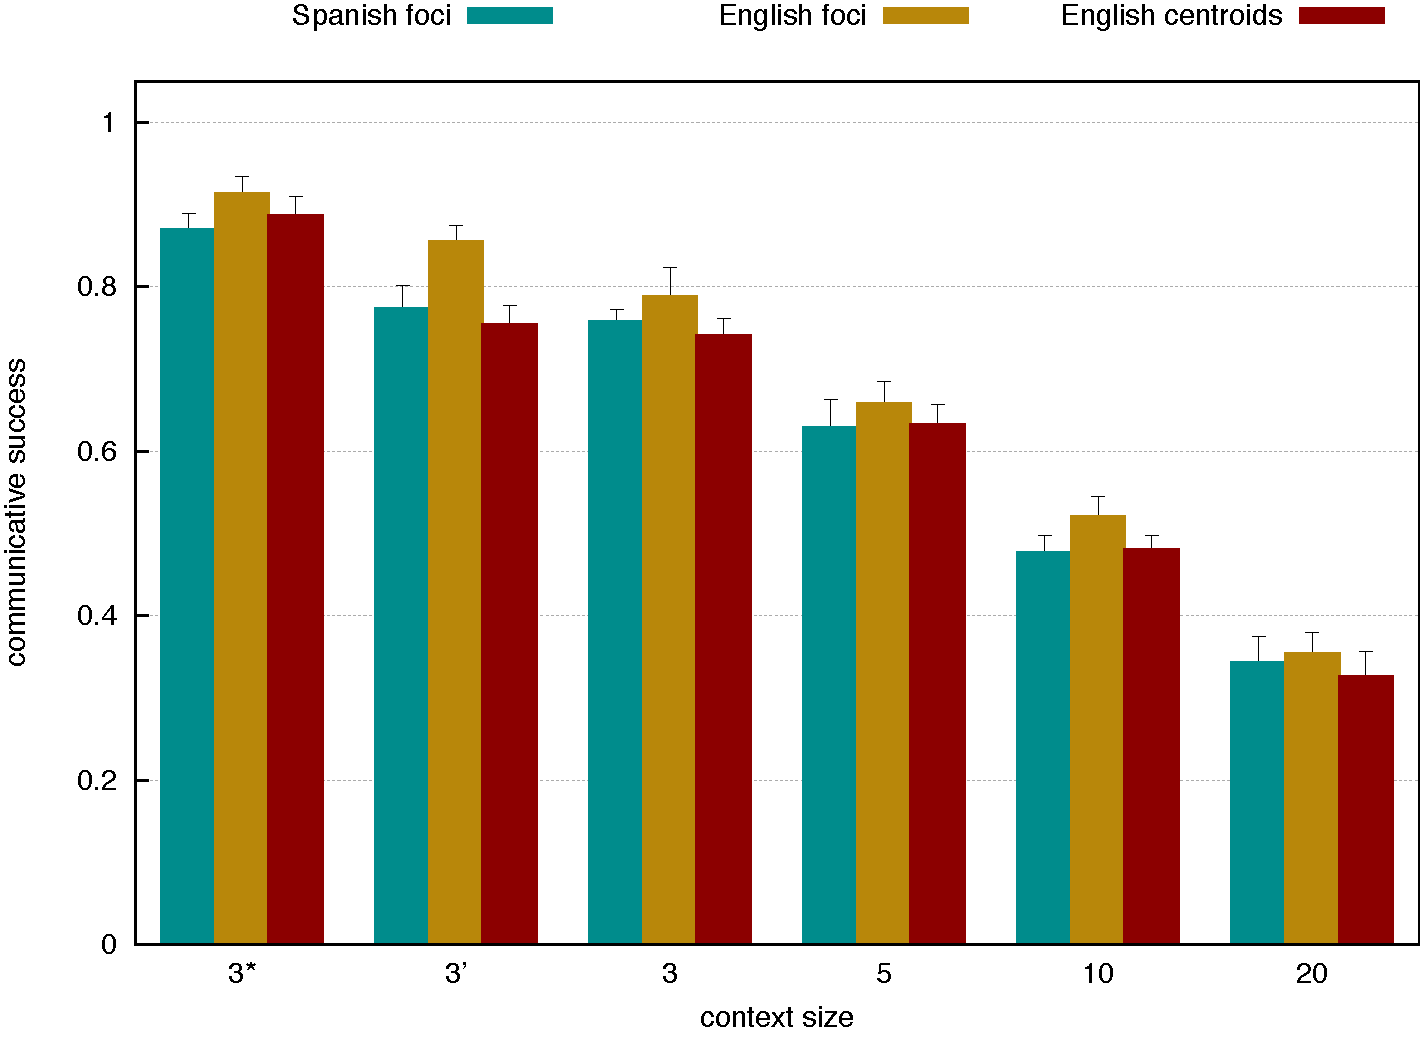
\includegraphics[width=\textwidth]{./basic-strategy/figures/baseline.pdf}
    \caption[The baseline communicative success of three predefined
    language systems]{The baseline communicative success of three
      predefined language systems: one is based on the Spanish foci
      \citep{lillo07locating} and the others are based on the foci and
      centroids of English \citep{sturges95location}. Baseline
      communicative success is inversely related to the context size
      increases. The context size for 3' is 3, but an additional
      constraint on the minimal interstimulus distance is
      imposed. Additionally, in 3* only the subset of Munsell chips
      that are faithfully reproducible are considered. These results
      are averaged over 8 runs.}
    \label{f:bcs-baseline}
  \end{center}
\end{figure}

The communicative success
\is{measures!communicative success}
\is{communicative success|see{measures}}
the ratio of
successful interactions in the last $cs_n$ games. The communicative
success has a maximum of 1 and minimum of 0. In all reported
experiments the value of $cs_n$ is set to 250.

\subsection{Results}

The communicative success of the baseline experiment is shown in
Figure \ref{f:bcs-baseline}. The more samples in one
context, the lower the corresponding communicative success. The
language system based on the English foci seems to perform slightly
better than the ones based on other language systems.


Imposing a minimal interstimulus distance of 50 in the CIE $L^*a^*b^*$
colour space (3' in Figure \ref{f:bcs-baseline}) does not
appear to have a significant impact on the resulting communicative
success, but the additional limitation to a particular subset of the
Munsell chip does (3* in Figure \ref{f:bcs-baseline}).

The main reason why some interactions still fail is that some samples
in a context could not be successfully discriminated because another
sample in the context was more similar to the prototype of the
category that the selected topic would belong to. For example, the
sample to the right in the context shown in Figure
\ref{f:bcs-failure-context}, will not be successfully named as
the middle sample is more similar to the prototype of the green colour
category.

\begin{figure}[htbp]
  \begin{center}
    
\includegraphics{./basic-strategy/figures/baseline-failure-context.pdf}
    \caption[Example context in which the basic colour strategy
    fails]{Example context in which the basic colour strategy
      fails. The sample to the right can not be successfully named as
      the middle sample is more similar to the prototype of the green
      colour category.}
    \label{f:bcs-failure-context}
  \end{center}
\end{figure}

\section{Conclusion}

In this chapter I have shown how the semantic and syntactic templates
of the \emph{basic colour strategy} can be defined. I have proposed
semantics that builds upon previous research, both in psychology and
artificial language evolution, and have extended it to accommodate for
several substrategies in which some dimensions of the colour domain
are more relevant as accounted by documented language systems. I have
proposed a mapping to language that encodes these semantics.
